% !TeX spellcheck = cs_CZ
%======================== Kapitola: Železniční zabezpečovací technika ============================
\chapter{Úvod}
\minitoc

  Základním požadavkem na železniční zabezpečovací zařízení je zajištění bezpečného provozu na 
  železnici. Tento požadavek je ohrožen vznikem poruch, čemuž nelze u reálných systémů zabránit 
  absolutně. Jak již bylo řečeno, tyto poruchy se nesmí projevit nebezpečným způsobem, čehož se 
  dosahuje vhodným návrhem systému. Z toho zdánlivě vyplývá, že na bezporuchovost (spolehlivost) 
  systému nemusí být kladeny příliš vysoké požadavky, neboť poruchy neohrožují bezpečnost dopravy.  

  Opak je však pravdou, protože lze očekávat, že vzrůstající poruchovost zařízení bude doprovázena 
  také vzrůstem obecné četnosti výskytu hazardních stavů a také četností výskytu hazardního stavu v 
  uvažovaném časovém okně (druhá porucha), což je podstatné u redundantních a reakčních systémů.
  
  Navíc případná nefunkčnost systému následkem poruchy znamená, že řízení provozu, který nemůže být 
  zastaven po celou dobu opravy systému, je nutné provádět bez jeho dohledu. Zodpovědnost je 
  přinejmenším částečně opět na člověku, který je navíc v této mimořádné situaci ještě náchylnější 
  k chybám. U zabezpečovacích zařízení tedy musíme požadovat i vysokou spolehlivost! Proto se v 
  následující kapitole budeme stručně věnovat popisu jednotlivých poruch.
  
  \section{Klasifikace poruch}
    \textbf{Chyba} je rozdíl mezi správnou a skutečnou hodnotou nějaké veličiny. V zařízení se 
    chyby mohou obecně objevit jako \emph{důsledek (projev) poruchy některé jeho součásti, 
    působením nějakého cizího vlivu} nebo \emph{selháním lidského činitele}. Za poruchy hardware se 
    považují všechna vybočení z předpokládaných vlastností stavebního prvku (součástky, dílu) 
    zařízení. Předpokládanými vlastnostmi prvků přitom jsou vlastnosti odpovídající příslušným 
    technickým podmínkám popisujícím jeho vlastnosti. Jako omyl lze označit každou lidskou činnost, 
    která může vést k nezamýšlenému chování zařízení. V širším slova smyslu se jako 
    \textbf{porucha} označují souhrnně všechny příčiny vedoucí k chybě, tj. poruch součásti, 
    cizí vliv i omyl.
      
\chapter{Bezpečnost a spolehlivost zabezpečovacích systémů}
 \section{Spolehlivost}
 \section{Bezpečnost}
    V různých publikacích je možné najít různé definice bezpečnosti. Například norma 
    EN~61508\footnote{Funkční bezpečnost elektrických/elektronických/programovatelných 
    elektronických systémů souvisejících s bezpečností (Functional safety of electrical/ 
    electronic/programmable electronic systems), obecná norma funkční bezpečnosti, která se opírá o 
    dvě základní koncepce - životní cyklus bezpečnosti a úroveň integrity bezpečnosti 
    (\texttt{SIL})} 
    definuje bezpečnost jako nepřítomnost netolerovaného rizika. Z této definice je zřejmé, že 
    bezpečnost je úzce spjatá s rizikem, a je nutné bezpečnost třeba chápat relativně. Když se 
    řekne, že řídicí systém je bezpečný, neznamená to jeho absolutní bezpečnost (ta je prakticky 
    nedosažitelná vzhledem na existenci objektivních faktorů, jako je například úroveň poznání, 
    technologická úroveň a limitované finanční prostředky), ale taková úroveň bezpečnosti, 
    která zodpovídá definovaným bezpečnostním požadavkům na tento řídicí systém. 

    Relativnost v pojímání bezpečnosti znamená posun od kvalitativního ke kvantitativnímu chápaní bezpečnosti.

    Kvalitativně je bezpečnost chápána jako schopnost řídicího systému zajistit omezení důsledků 
    poruch řídicích systému v daných podmínkách a v daném časovém intervalu. Matematicky je možné 
    kvalitativní bezpečnost řídicího systému vyjádřit jako 
    \begin{equation}
      E_H = 0,
    \end{equation}
    kde \(E_H\) je množina nebezpečných stavů, které jsou důsledkem výskytu pravděpodobných poruch 
    řídicího systému. Pravděpodobná porucha je taková porucha z množiny všech poruch, jejichž 
    výskyt během provozu řídicího systému je nutné předpokládat (vzhledem na požadovanou úroveň 
    bezpečnosti řídicího systému).
	
    Kvantitativně je bezpečnost řídicího systému chápána jako pravděpodobnost nepřítomnosti
    jakéhokoliv nebezpečného stavu v řídicím systému v daných podmínkách a v daném časovém
    intervalu. Je zřejmé, že i když pravděpodobnost nebezpečného stavu řídicího je malá, neznamená
    to, že se nebezpečný stav nemůže vyskytnou v nejbližším časovém intervalu, Matematicky je možné
    kvantitativní bezpečnost vyjádřit tak, že
    \begin{equation}
      P_{HT}(t)\geq P_{HT}(t)>0,
    \end{equation}
    kde \(P_{HT}(t)\) je pravděpodobnost tolerovaného nebezpeční řídicího systému a \(P_{HR}(t)\)
    je reálná pravděpodobnost nebezpeč\-ného stavu řídicího systému.
	 
    Na kvantitativním hodnocení bezpečnosti řídicího systému je v podstatě možné uplatnit stejné 
    teoretické postupy, jako při hodnocení spolehlivosti technických systémů. Zásadní rozdíl je v 
    tom, že při hodnocení spolehlivosti standardních řídicích systémů se obvykle rozlišují dva 
    stavy - bezporuchový stav a poruchový stav, a k těmto dvěma stavům se vztahují také 
    kvantitativní ukazatele spolehlivosti. Při hodnocení bezpečnosti řídicích systémů musíme 
    uvažovat s dvěma druhy poruchových stavů - bezpečným a nebezpečným poruchovým stavem. 
    Bezpečnost řídicího systému se potom vyjadřuje pomocí ukazatelů bezpečnosti (například 
    pravděpodobnost výskytu nebezpečné poruchy, intenzita nebezpečných poruch, ...).

    Při kvantitativním hodnocení důsledků poruch na bezpečnost řídicího systému se obvykle k 
    hodnoceným řídicím systémům přistupuje jako k neobnovovaným objektům, protože z pohledu 
    bezpečnosti jsou důležité dva stavy (bezpečný, nebezpečný) a analýza končí výskytem nebezpečné 
    poruchy (může jít o jednu poruchu, nebo o kombinaci více poruch, které nejsou individuálně 
    nebezpečné). To znamená, že od uvedení řídicího systému do provozu, až po výskyt nebezpečné 
    poruchy, se může řídicí systém střídavě nacházet ve funkčním, nebo nefunkčním stavu (nefunkční 
    ještě neznamená nebezpečný). Z tohoto důvodu ukazatele bezpečnosti jsou podobné ukazatelům 
    bezporuchovosti neobnovovaných objektů. 
  
    \subsection{Základní legislativa}
      \begin{itemize}
        \item \textbf{EN 61508} - \emph{základní všeobecná norma pro SRCS}; pojednává o funkční
              bezpečnosti elektrických/elektronických/programovatelných elektronických systémů
              souvisejících s bezpečností (Functional safety of electrical/electronic/programmable
              electronic systems), obecná norma funkční bezpečnosti, která se opírá o dvě základní
              koncepce - životní cyklus bezpečnosti a úroveň integrity bezpečnosti (\texttt{SIL})
              \begin{itemize}
                \item EN 61508-1: Všeobecné požadavky
                \item EN 61508-2: Požadavky na elektrické / elektronické / programovatelné
                                  elektronické systémy související s bezpečností
                \item EN 61508-3: Požadavky na SW
                \item EN 61508-4: Definice a zkratky
                \item EN 61508-5: Příklady metod určování úrovně integrity bezpečnosti
                \item EN 61508-6: Metodické pokyny na používání EN 61508-2, STN EN 61508-3
                \item EN 61508-7: Přehled technik a opatření
              \end{itemize}
        \item \textbf{EN 50126}: Railway applications – The specification and demonstration of
              reliability, availability, maintainability and safety (RAMS)
              \begin{itemize}
                \item Part 1: Basic requirements and generic process. 1999
                \item Part 2: Guide to the application of EN 50126-1 for safety. 2007
                \item Part 3: Guide to the application of EN 50126-1 for rolling stock RAMS. 2008  
              \end{itemize}
              Zabývá se specifikací parametrů RAMS (spolehlivost, pohotovost, udržovatelnost,
              a bezpečnost) obecně pro všechny železniční systémy, reaguje na skutečnost, že
              naléhavost požadavků na bezpečnost funkce jednotlivých železničních systémů je různá
              a lze je tedy splňovat s různou pravděpodobností jejich selhání. Také zavádí pojem
              \emph{integrita bezpečnosti (safety integrity - celistvost, úplnost, neporušenost
              bezpečnosti)}, který definuje jako pravděpodobnost, s níž systém uspokojivě splní
              požadované bezpečnostní funkce, za všech stanovených podmínek a ve stanoveném časovém
              období. Jde o to, do jaké míry může být pro bezpečnost relevantní funkce narušena
              např. poruchami vlastního zařízení, omyly obsluhy, vnějším rušením atd.
        \item \textbf{EN 50128}: Railway applications – Communication, signalling and processing
              systems – Software for railway control and protection systems. 2003          
        \item \textbf{EN 50129}: Railway applications – Communication, signalling and processing
              systems – Safety-related electronic systems for signalling. 2011
              Modifikovaně byl pojem integrita bezpečnosti přenesen i do této normy pro železniční
              zabezpečovací systémy. I klasická zabezpečovací technika bez velkého zdůrazňování
              respektovala, že nejsou na všechna zařízení kladeny stejně důrazné bezpečnostní
              požadavky (kategorie zařízení, vedlejší tratě/hlavní tratě, zařízení pro ČD/zařízení
              pro vlečky, staniční zařízení/spádoviště atd.). Uvidíme dále, že pojmu integrita
              bezpečnosti je pro zabezpečovací zařízení dominantně obsažena oblast, kterou běžně v
              této technice označujeme(a také normá EN 50129 ji tak označuje ve své základní části)
              termínem technická bezpečnost. Úvahy okolo integrity bezpečnosti zde sledujeme
              odděleně od úvah o technické bezpečnosti (přes jejich podobnost) pro jejich výhodnost
              zejména v úvodních fázích projektu nového systému (zařízení, výrobku, atd.)
        \item \textbf{EN 50159: Railway applications – Communication, signalling and processing
              systems - Safety-related communication in transmission systems. 2010}            
      \end{itemize}
    
      Vyjmenované normy se poněkud liší v definici termínu \emph{bezpečnost}:  
      \begin{itemize}
        \item Bezpečnost (Safety) – nepřítomnost nepřijatelných úrovní rizika poškození (EN50129)
        \item Bezpečnost (Safety) – nepřítomnost nepřijatelného rizika. (EN61508)
        \item Bezpečnost při poruše (Fail Safe) – vlastnost konstrukce objektu zabraňující,
              aby jeho poruchy způsobili nebezpečné poruchové stavy. (IEC 50 (191))
        \item Kvalitativní bezpečnost – schopnost systému zajistit omezení důsledku poruch
              systému v daných podmínkách a v daném časovém intervale.
        \item Kvantitativní bezpečnost – pravděpodobnost nepřítomnosti jakéhokoliv
              nebezpečného stavu v systéme v daných podmínkách a v daném časovém intervale.
      \end{itemize}

    \subsection{Ukazatel bezpečnosti}
      \fbox{Pravděpodobnost bezpečného provozu} je pravděpodobnost, že objekt může bezpečně plnit 
      požadovanou funkci v daných podmínkách v časovém intervalu \(t_1,\, t_2\).
      \begin{equation}
        R_S(t_1,\, t_2) = 1- F_H(t_1,\, t_2),
      \end{equation}
      kde \(F_H(t_1,\, t_2)\) je distribuční funkce, která naopak vyjadřuje pravděpodobnost, že
      objekt nemůže bezpečně plnit požadovanou funkci k daným podmínkám v časovém intervalu
      \(t_1,\, t_2\).
      \begin{equation}
        F_H(t_1,\, t_2) = \int_{t_1}^{t_2}f_H(t)\cdot\dd{t},
      \end{equation}
      kde \(f_H(t)\) je hustota pravděpodobnosti nebezpečné poruchy objektu. 

      \fbox{Intenzita nebezpečných poruch} \(\lambda_H(t)\) definujme jako limitu poměru podmíněné
      pravděpodobnosti, že časový okamžik vzniku nebezpečné poruchy objektu \(T\) padne do daného
      časového intervalu \(t,\, t+\Delta t\), přičemž délka časového intervalu \(\Delta
      t\rightarrow0\)
      \begin{equation}\label{DZT:eq_def_lambdaH}
        \lambda_H=\frac{f_H(t)}{R_S(t)}.
      \end{equation}

      Protože nebezpečné poruchy jsou méně časté, zkoušky na určení požadovaných ukazatelů
      bezpečnosti by bylo třeba provádět dlouhodobě, což je prakticky nemožné. 
    
  \section{Integrita bezpečnosti}
    Všeobecně je možné konstatovat, že SRCS realizuje řídící i ochranné funkce (obr.
    \ref{DZT:fig_DZT_SRCS_fce}). Jelikož selhání řídicí funkce může způsobit ohrožení bezpečnosti,
    je třeba i tyto funkce považovat za bezpečnostní.
    \begin{figure}[hb!]
      \centering
      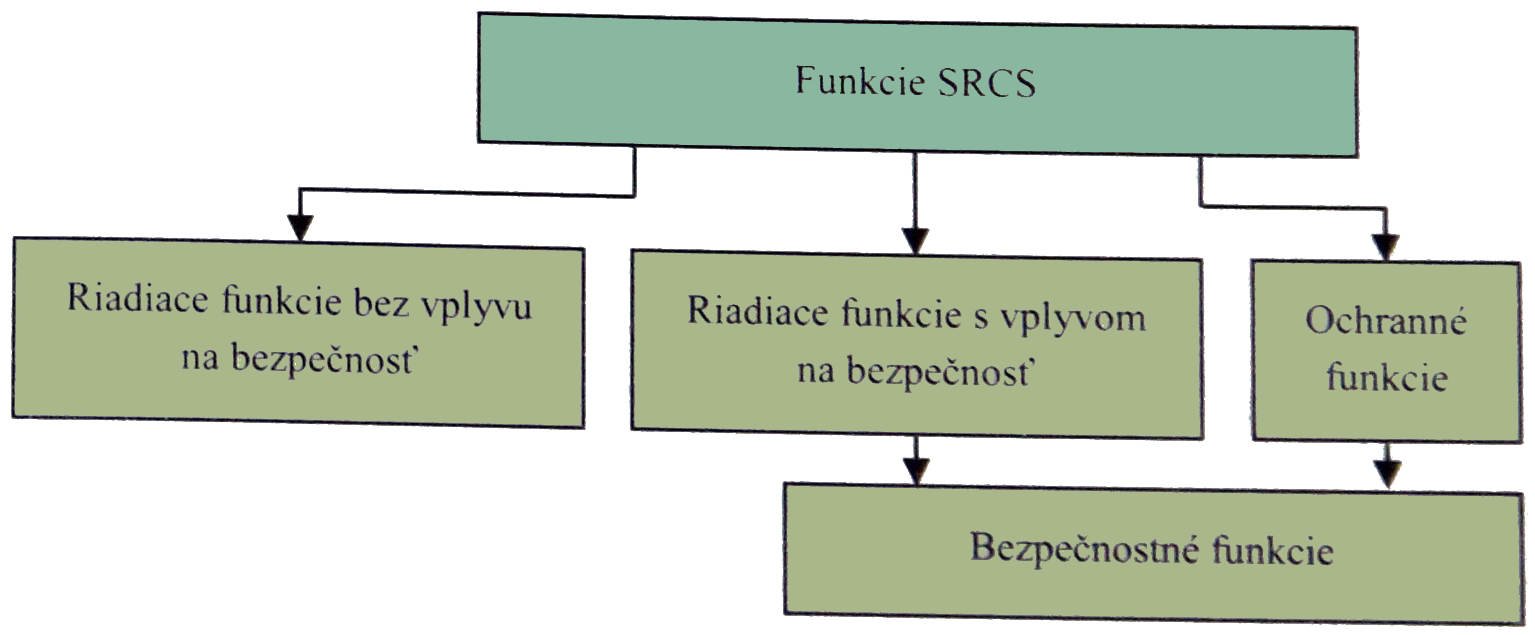
\includegraphics[width=1\linewidth]{DZT_SRCS_fce.jpg}
      \caption{Vztah mezi bezpečnostními funkcemi a moduly SRCS}
      \label{DZT:fig_DZT_SRCS_fce}
    \end{figure}    
    Bezpečnostní funkce jsou definované na základě analýzy rizik jako technická opatření na snížení
    rizika spojeného s konkrétními nebezpečí na tolerovatelnou úroveň. Účinnost bezpečnostní funkce
    se určuje pomocí úrovně integrity bezpečnosti \emph{(\texttt{SIL} - safety integrity level)}. 
    
    Norma \emph{EN 61508} definuje integritu bezpečnosti jako pravděpodobnost, že SRCS bude plnit 
    požadované bezpečné funkce za všech stanovených podmínek v rámci stanoveného operačního 
    prostředí a během stanoveného časového období. Všeobecně lze konstatovat, že čím je integrita
    bezpečnosti SRCS větší, tím je menší pravděpodobnost selhání bezpečností funkce realizovaných
    SRCS.  
    
    Integrita bezpečnosti se skládá ze dvou částí a to:
    \begin{itemize}
      \item \emph{integrity bezpečnosti proti systematickým poruchám}: jde o nekvantifikovatelnou
            část integrity bezpečnosti, která souvisí s nebezpečnými systematickými poruchami 
            hardware a software; integrity bezpečnosti proti systematickým poruchám se dosahuje
            především opatřeními na předcházení chybám a poruchám; vzhledem k tomu, že jde o 
            nekvantifikovatelnou část integrity bezpečnosti, je vhodnější chápat integritu 
            bezpečnosti jako vlastnost a né jako pravděpodobnost; hodnocení integrity bezpečnosti
            proti systematickým chybám a poruchám se realizuje kontrolou dodržování opatření
            předcházejících chybám a poruchám, mezi které patří také důsledné testování korektní
            realizace bezpečnostních funkcí; 
      \item \emph{integrity bezpečnosti proti náhodným poruchám}: jde o kvantifikovatelnou část
            integrity bezpečnosti, která se týká náhodných poruch hardware vyplývajících z konečné
            bezporuchovosti použitých součástek; hodnocení integrity bezpečnosti proti náhodným
            poruchám se realizuje prostřednictvím pravděpodobnostních výpočtů.
    \end{itemize}
    
    Aby se dosáhla požadovaná integrita bezpečnosti, musí být splněné požadavky na integritu proti 
    systematickým poruchám i náhodným poruchám. 
    
    \subsection{Úroveň integrity bezpečnosti}
      Úroveň integrity bezpečnosti (\emph{Safety Integrity Levels - \texttt{SIL}}) se dělí podle EN 
      50129
      do čtyř kategorií - úroveň 4 (\texttt{SIL} 4) je nejvyšší, úroveň 1 (\texttt{SIL} 1) je 
      nejnižší.  Pokud se
      objevuje úroveň \texttt{SIL} 0, značí to, že se jedná o systém na které nejsou kladeny žádné
      bezpečnostní požadavky (ve smyslu zabezpečovací techniky)
      
      Proto, aby SRCS mohl být zařazen do odpovídající úrovně bezpečnosti \texttt{SIL}, musí 
      vyhovovat
      těmto faktorům:
      \begin{itemize}
        \item naplnění podmínek řízení kvality, 
        \item naplnění podmínek řízené bezpečnosti,
        \item splnění požadavků na technickou bezpečnost, 
        \item dosažení kvantitativního cíle
      \end{itemize}
      
      Jak patrno, splnění kvantitativního ukazatele samo o sobě neznamená, že bylo dosaženo
      odpovídající úrovně bezpečnosti. To platí ovšem i naopak - splnění tří předchozích podmínek
      (řízení kvality, řízení bezpečnosti a technické bezpečnosti) nezaručuje, že bylo dosaženo
      kvantitativních cílů a nelze tedy tvrdit, že zařízení lze zařadit do odpovídající skupiny
      \texttt{SIL} (\ref{DZT:fig_EN50129_SIL_techniques}).
      
      \begin{figure}[ht!]% Relationship between \texttt{SIL}s and techniques
        \centering
        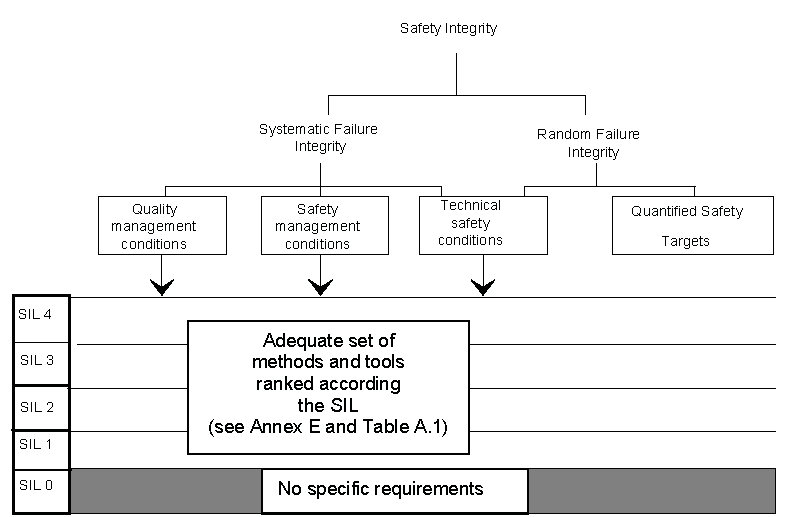
\includegraphics[width=0.95\linewidth]{EN50129_SIL_techniques.pdf}
        \caption{Vztah mezi \texttt{SIL} úrovní a technikami jejich dosažení}
        \label{DZT:fig_EN50129_SIL_techniques}
      \end{figure}
      
      Žádná z norem \texttt{CENELEC} nepředepisuje, které zařízení musí být jaké úrovně. Toto 
      určení je 
      ponecháno na provozovateli, resp. regulátorovi, vyplyne také z provedených analýz rizik 
      a hazardů.
      
      Následující tabulka shrnuje definované úrovně integrity bezpečnosti a zároveň dává do
      souvislosti s tolerovatelnými četnostmi hazardů. \texttt{SIL} jsou tedy prostředkem přiřazení
      kvalitativních přístupů (pro vyloučení systematických poruch) ke kvantitativnímu přístupu
      (pro řízení náhodných poruch), neboť systematické poruchy nelze kvantifikovat.
      \begin{table}[h]
        \centering
        \begin{tabular}{|c|c|}
          \hline
           Úroveň integrity &  Tolerovatelná četnost hazardu            \\
             bezpečnosti \texttt{SIL} &  THR [za hodinu a funkci]       \\ \hline\hline 
              4        & \(10^{-9}\leq THR < 10^{-8}\)                  \\ \hline
              3        & \(10^{-8}\leq THR < 10^{-7}\)                  \\ \hline
              2        & \(10^{-7}\leq THR < 10^{-6}\)                  \\ \hline
              1        & \(10^{-6}\leq THR < 10^{-5}\)                  \\ \hline
        \end{tabular}
        \caption{\texttt{SIL} tabulka: Funkce, jejichž kvantitativní požadavky by převyšovaly 
                 hranici \(10^{-9}\), která se zdánlivě nelogicky objevuje u \texttt{SIL4}, vyžaduje
                 podle normy \texttt{EN~50129} zvláštní technická nebo provozní opatření pro 
                 dosažení tak mimořádného cíle.}
      \end{table}
       
      \begin{enumerate}
        \item Z normy jasně vyplývá rozdělení na dvě skupiny \texttt{SIL 1,2} vs. \texttt{SIL 3,4}, 
              u nichž je výrazný rozdíl v požadavcích, které je potřeba splnit, aby SRCS mohl 
              patřit do dané skupiny. To je velmi dobře patrné z tabulek v příloze \texttt{E} normy 
              \texttt{EN 50129}, která se zabývá technikami a opatřeními pro řízení náhodných a 
              systematických poruch. 
        \item Druhým důležitým faktem je poněkud odlišná definice chápání úrovní \texttt{SIL} v 
              EN~61508. \emph{Funkční bezpečnost elektrických, elektronických, programovatelných
              elektronických systémů souvisejících s bezpečností}. Tato norma je obecnou normou pro
              průmyslové elektronické systémy, z níž vycházejí normy EN~50126, EN 50~129 atd.
              jakožto specifické normy pro železniční aplikace. Důležitou odlišností ve specifikaci
              \texttt{SIL}, viz tab. 2 a 3 v první části této normy (EN~61508-1). Nicméně tabulka 3 
              pro
              režim provozu s vysokým, resp. nepřetržitým vyžádáním odpovídá tabulce v normě
              EN~50129. Avšak i pro tyto systémy se zde jeví určitá odlišnost v požadavcích na
              zajištění dané \texttt{SIL}. Norma EN~61508 je zaměřena pouze na \emph{funkční 
              bezpečnost},
              není zde zahrnutý požadavek na bezpečnou reakci na ojedinělé náhodné poruchy. S
              poruchami se samozřejmě pracuje, mají být provedena opatření k jejich maximálnímu
              potlačení - četnosti i následku, nicméně může stačit, když systém je schopen poruchy
              detekovat a dát o nich vědět (např. obsluze). Závěrem nutno dodat, že je potřeba
              určité obezřetnosti k tvrzení, že systém splňuje daný \texttt{SIL}. Tento údaj musí 
              být
              doplněn specifikací, která norma byla při klasifikaci použita.
      \end{enumerate}